\section{The physical sensing budget}
\label{sec:budget}

\begin{figure*}[t]
\centering
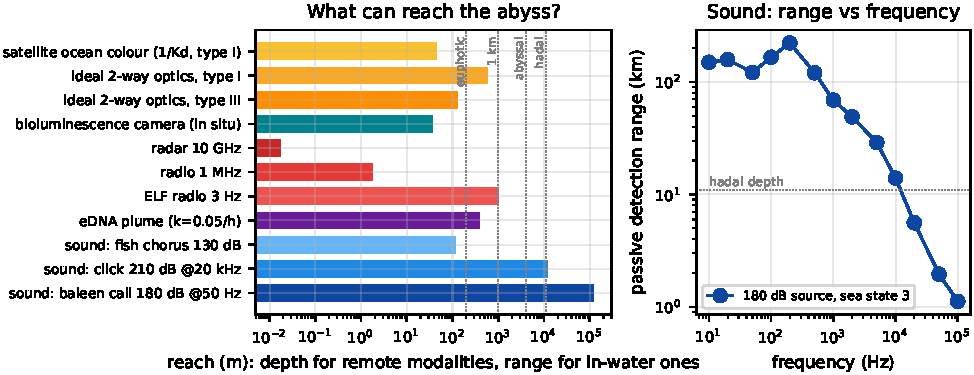
\includegraphics[width=\textwidth]{figures/budget.pdf}
\caption{Left: how far each modality reaches (depth for remote sensing, range
for in-water sensors), log scale, against the euphotic, 1\,km, abyssal and
hadal marks. Right: passive detection range of a 180\,dB source versus
frequency (sea state 3, hybrid spreading); only sound below a few hundred
hertz crosses the full water column with margin.}
\label{fig:budget}
\end{figure*}

Figure~\ref{fig:budget} summarises the closed forms; all parameters are in the
configuration.

\paragraph{Light.} Irradiance decays as $E(z) = E_0 e^{-K_d z}$. In the
clearest Jerlov type~I water ($K_d = 0.022$\,m$^{-1}$) the 1\% euphotic depth
is \EuphoticI\,m, and in coastal type~III it is \EuphoticIII\,m. Ocean-colour
imagery integrates about one attenuation length, \OceanColourDepth\,m. Even an
ideal detector with a $10^{-11}$ dynamic range on a round trip (sunlight down,
reflection up) would reach \OpticsReachI\,m in type~I and \OpticsReachIII\,m in
type~III --- an order of magnitude short of the abyss. In situ, a $10^{10}$
photon bioluminescent flash is visible to a 10\,cm$^2$ camera at
\BiolumRange\,m: cameras see what swims past, nothing more.

\paragraph{Radio and radar.} The skin depth $\delta = 1/\sqrt{\pi f \mu_0
\sigma}$ with $\sigma = 4$\,S/m is \SkinRadar\,mm at 10\,GHz, \SkinMHz\,cm at
1\,MHz and \SkinELF\,m at 3\,Hz; with a generous 60\,dB link margin the 3\,Hz
extremely-low-frequency band used to signal submarines reaches
\ReachELF\,km. No satellite electromagnetic sensor sees below the mixed layer.

\paragraph{Sound.} The passive sonar equation $\mathrm{SL} - \mathrm{TL}(r,f) -
(\mathrm{NL}(f) - \mathrm{DI}) \geq \mathrm{DT}$ with Thorp absorption
(\ThorpFifty\,dB/km at 50\,Hz, \ThorpTwentyK\,dB/km at 20\,kHz) and Wenz noise
at sea state~3 gives the ranges of Table~\ref{tab:sound}. A 180\,dB baleen
call at 50\,Hz is detectable at \RangeBaleenSph\,km with spherical spreading
and \RangeBaleenHyb\,km when spreading becomes cylindrical beyond the water
depth; a 210\,dB odontocete click at 20\,kHz is absorption-limited to
\RangeClick\,km; a 130\,dB fish chorus at 300\,Hz reaches \RangeFish\,m and a
100\,dB soft-bodied animal only \RangeQuiet\,m. Sound is the one modality that
crosses the abyss, and it does so for loud, low-frequency callers; the
quietest animals are audible only from a few metres, which is where an
instrumented lander or ROV must be.

\begin{table}[t]
\centering\small
\begin{tabular}{lrrr}
\toprule
source & SL (dB) & $f$ & range \\
\midrule
baleen call & 180 & 50\,Hz & \RangeBaleenHyb\,km \\
odontocete click & 210 & 20\,kHz & \RangeClick\,km \\
invertebrate snap & 150 & 5\,kHz & \RangeSnap\,km \\
fish chorus & 130 & 300\,Hz & \RangeFish\,m \\
soft body, quiet & 100 & 1\,kHz & \RangeQuiet\,m \\
\bottomrule
\end{tabular}
\caption{Passive detection ranges (sea state 3, moderate shipping, DT 10\,dB,
hybrid spreading with a 4\,km transition).}
\label{tab:sound}
\end{table}

\paragraph{Environmental DNA.} A source shedding $10^8$ copies/h into a
0.05\,m/s current with eddy diffusivity 1\,m$^2$/s and decay 0.05\,h$^{-1}$ is
detectable at 0.01 copies/L up to \EdnaFootprint\,m downstream, and the
sample's memory is $1/k = \EdnaMemory$\,h. eDNA thus integrates a
neighbourhood of hundreds of metres over a day --- a superb presence sensor,
but one that identifies only what has a reference sequence, so for a truly new
species it returns ``unassigned'' rather than a description.

\paragraph{What the satellite is for.} Altimetry-derived bathymetry, surface
chlorophyll and thermal fronts do not see animals, but they predict where
animals concentrate (seamounts, canyons, upwelling). We carry this into
Section~\ref{sec:survey} as a habitat prior of variable reliability: the
satellite tells the ship where to lower the hydrophone.
